\begin{frame}{CS Background}
    \begin{block}{Turing Machines}
        \begin{figure}
            \centering
            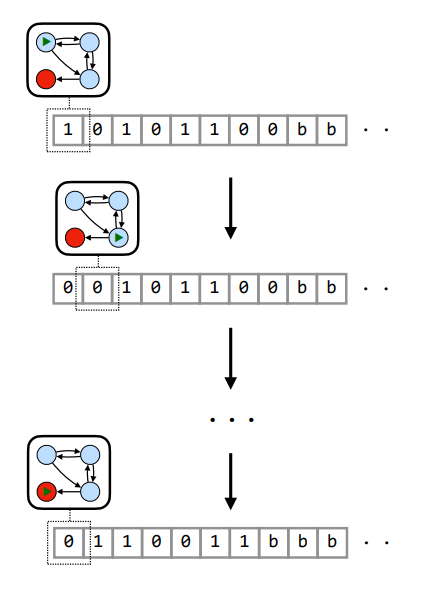
\includegraphics[height=5cm]{TM.png}
            \caption{Graphical representation of a TM}
            \label{fig:my_label}
        \end{figure}
    \end{block}
\end{frame}

\begin{frame}{CS Background}
\begin{block}{Turing Machines}
Formal definition of a Turing Machine:
    \begin{itemize}
        \item A Turing machine $M$ is a 4-tuple $M = (Q,\Sigma, q_0,\delta) $ where:
        \begin{itemize}
            \item $Q$ is a finite nonempty set of states.
            \item $\Sigma$ is a finite nonempty set of symbols.
            \item $q_0\in Q$ is the initial state of $M$
            \item $\delta: (Q\times \Sigma) \nrightarrow (\Sigma \times \{L,R\}\times Q)$ is a partial transition function determining the symbol written on the tape, the movement of the read-write head, and the next state of the $M$.
        \end{itemize}
    \end{itemize}
\end{block}
\end{frame}

\begin{frame}{CS Background}
    \begin{block}{Additional Assumptions on TM $M$}
    
    \begin{enumerate}
        \item $\Sigma = \{0,1,b\}$
        \item If and when $M$ halts on an input, the tape will contain an output string $s\in \{0,1\}^*$ followed by all blank symbols, and the pointer will be set to the start of the tape.
    \end{enumerate}
    Assumptions do not affect the computational capabilities of $M$.
    \end{block}
\end{frame}
    
\begin{frame}{CS Background}
    \begin{block}{Turing Machines as Partial Functions}
    Any computation performed by a TM $M$ can be represented as
    \begin{equation*}
        \phi_M:\{0,1\}^* \nrightarrow \{0,1\}^*
    \end{equation*}
    and $\phi_M(x) = y$ indicates that $M$ started with input program $x$ yields the output string $y$.
    \end{block}
    \begin{block}{Universal TM}
    There exist Universal Turing Machines (UTM) such that given a UTM $U$ and any TM $M$, there exists an interpreter program $\sigma_{U,M}$ such that
    \begin{equation*}
        \phi_U(\sigma_{U,M},x) = \phi_M(x)
    \end{equation*}
    \end{block}
\end{frame}

\begin{frame}{CS Background}
\begin{block}{The Print function, an example}
\begin{itemize}
	\item There exists a FPGA (Field-programmable-gate-array) which constitutes a circuit capable of parroting back any binary string fed to it.
	\item This computer is also capable of printing out a binary string.
\end{itemize}
\end{block}
\end{frame}

\begin{frame}{CS Background}
\begin{block}{The Print function, an example}
	\begin{itemize}
		\item $\phi_D$ UTM which models my personal computer
		\item $\phi_M$ TM which models a "print" FPGA
		\item $x$ binary string which $\phi_M$ can print
		\item $\sigma_{D,M}$ interpreter program
		\item $(\sigma_{D,M},x)$ input to my UTM $\phi_D$
	\end{itemize}
\end{block}
\end{frame}

\begin{frame}{CS Background}
\begin{block} {TM input}
\begin{itemize}
	\item The input to a TM is not generally the input to a program
	\item The input to a TM is the program itself, along with any necessary parameters
\end{itemize}
\end{block}
\end{frame}

\begin{frame}{CS Background}
    \begin{block}{Computability}
    \begin{itemize}
        \item Church Turing Thesis: A function can be calculated by a sequence of formal operations if and only if it is computable by a Turing Machine.
       \item Physical Church Turing Thesis: Any function implemented by a physical process can also be implemented by a Turing Machine
    \end{itemize}
    \end{block}
\end{frame}



%%%%%%%%%%%%%%%%%%%%%%%%%%%%%%%%%% Realization of a TM%%%%%%%%%%%%%%%%%%
\begin{frame}{Realizations of a TM}
    \begin{block}{Realizations and Computable Realizations}
    \begin{itemize}
        \item \textbf{Physical Realization}: A physical process consistent with the laws of thermodynamics and whose dynamics correspond to the input-output map of a TM $M$
        \item \textbf{Computable Realization}: A physical realization of a TM $M$ whose generated heat on an input program $x$ can be determined by a computable function
    \end{itemize}
    \end{block}
\end{frame}

\begin{frame}{Realizations of a TM}

    \begin{figure}
            \centering
            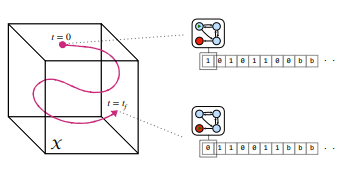
\includegraphics{System.png}
            \label{fig:my_label2}
        \end{figure}
    
\end{frame}